\documentclass[11pt]{article}

\usepackage{fullpage} 
\usepackage{hyperref}
\usepackage{amsmath}
\usepackage{amssymb}
\usepackage{amsthm}
\usepackage{graphicx}
\usepackage{pgf}
\usepackage{tikz}
\usetikzlibrary{arrows,automata}
\usepackage{indentfirst}

\newcommand{\question}[2] {\vspace{0.3in}\noindent{\subsection*{Question #1. #2} \vspace{0.15in}}}

\renewcommand{\part}[1] {{\vspace{0.15in}\noindent\textbf (#1)} \vspace{0.10in}}



%  ----------------------------------------------------------------
%                         Start here
% ----------------------------------------------------------------
 
\begin{document}

\title{Assignment \#4} %Replace X with the appropriate number
\author{\Large Gustavo Estrela de Matos\\ %Replace with your name
CSCE 433: Formal Languages and Automata} %If necessary, replace with your course number and title
\date{\today} 

\maketitle

\question{1}{}
\par To build both NFAs we are going to use the bottom-up approach

\part{a}
\begin{itemize}
    \item{$0:$
        
    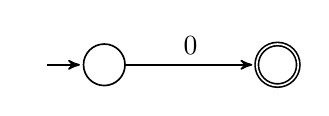
\begin{tikzpicture}[->,>=stealth',shorten >=1pt,auto,node distance=2.2cm, semithick, initial text={}]
  
    \tikzstyle{every state}=[fill=white,draw=black,text=black, minimum size=15pt]

    \node[initial,state]    (0)              {};
    \node[accepting, state] (1) [right of=0] {};
 
    \path (0) edge node {$0$} (1)
                                      
    ;                      
    \end{tikzpicture}    
    }

    \item{$1:$
        
    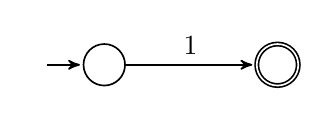
\begin{tikzpicture}[->,>=stealth',shorten >=1pt,auto,node distance=2.2cm, semithick, initial text={}]
  
    \tikzstyle{every state}=[fill=white,draw=black,text=black, minimum size=15pt]

    \node[initial,state]    (0)              {};
    \node[accepting, state] (1) [right of=0] {};
 
    \path (0) edge node {$1$} (1)
                                      
    ;   
    \end{tikzpicture}    
    }

    \item{$11:$

        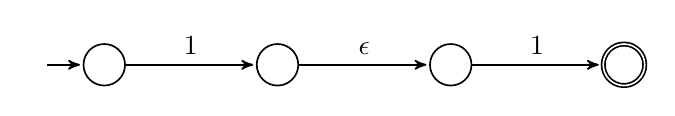
\begin{tikzpicture}[->,>=stealth',shorten >=1pt,auto,node distance=2.2cm, semithick, initial text={}]
  
        \tikzstyle{every state}=[fill=white,draw=black,text=black, minimum size=15pt]

        \node[initial,state]    (0)              {};
        \node[state]            (1) [right of=0] {};
        \node[state]            (2) [right of=1] {};
        \node[accepting, state] (3) [right of=2] {};
            
        \path (0) edge node {$1$} (1)
        (1) edge node {$\epsilon$} (2)
        (2) edge node {$1$} (3)
                                      
    ;    
    \end{tikzpicture}    
    }

    \item{$(11)^*:$
 
        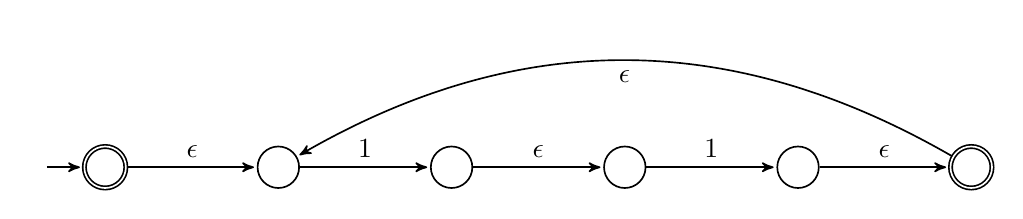
\begin{tikzpicture}[->,>=stealth',shorten >=1pt,auto,node distance=2.2cm, semithick, initial text={}]
  
        \tikzstyle{every state}=[fill=white,draw=black,text=black, minimum size=15pt]
    
        \node[initial, accepting, state] (4)     {};
        \node[state]            (0) [right of=4] {};
        \node[state]            (1) [right of=0] {};
        \node[state]            (2) [right of=1] {};
        \node[state]            (3) [right of=2] {};
        \node[accepting, state] (5) [right of=3] {};
            
        \path 
        (4) edge node {$\epsilon$} (0)
        (0) edge node {$1$} (1)
        (1) edge node {$\epsilon$} (2)
        (2) edge node {$1$} (3)
        (3) edge node {$\epsilon$} (5)
        (5) edge [bend right=30] node {$\epsilon$} (0)
    ;    
    \end{tikzpicture}           
        
    }

    \item{$0 + 1:$

        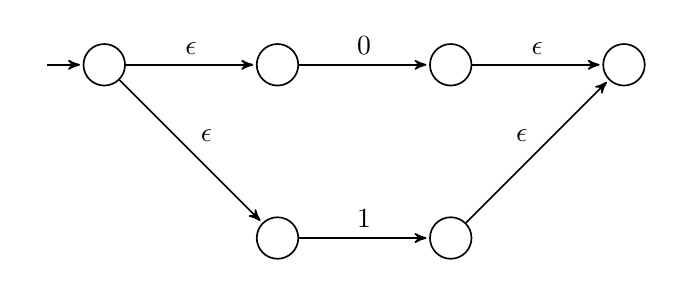
\begin{tikzpicture}[->,>=stealth',shorten >=1pt,auto,node distance=2.2cm, semithick, initial text={}]
  
        \tikzstyle{every state}=[fill=white,draw=black,text=black, minimum size=15pt]
    
        \node[initial, state]   (6)                  {};
        \node[state]            (7)  [right of = 6]  {};
        \node[state]            (8)  [below of = 7]  {};
        \node[state]            (12) [right of = 8]  {};
        \node[state]            (9)  [right of = 7]  {};
        \node[state]            (10) [right of = 9]  {};
            
        \path 
        (6)  edge node {$\epsilon$} (7)
        (6)  edge node {$\epsilon$} (8)
        (7)  edge node {$0$}        (9)
        (9)  edge node {$\epsilon$} (10)
        (8)  edge node {$1$}        (12)
        (12) edge node {$\epsilon$} (10)
    ;    
    \end{tikzpicture}           
    }

    \item{$(0 + 1)(11)^*:$
        
        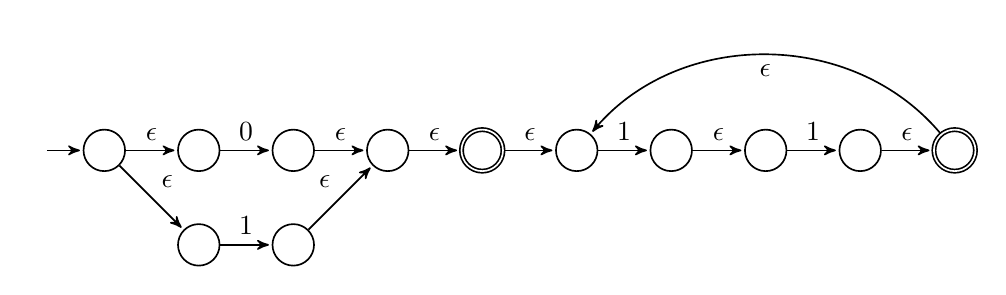
\begin{tikzpicture}[->,>=stealth',shorten >=1pt,auto,node distance=1.2cm, semithick, initial text={}]
  
        \tikzstyle{every state}=[fill=white,draw=black,text=black, minimum size=15pt]
    
        \node[initial, state]   (6)                  {};
        \node[state]            (7)  [right of = 6]  {};
        \node[state]            (8)  [below of = 7]  {};
        \node[state]            (12) [right of = 8]  {};
        \node[state]            (9)  [right of = 7]  {};
        \node[state]            (10) [right of = 9]  {};
         
        \node[accepting, state]            (4)  [right of=10]   {};
        \node[state]            (0)  [right of=4]    {};
        \node[state]            (1)  [right of=0]    {};
        \node[state]            (2)  [right of=1]    {};
        \node[state]            (3)  [right of=2]    {};
        \node[accepting, state] (5)  [right of=3]    {};
   
        \path 
        (6)  edge node {$\epsilon$} (7)
        (6)  edge node {$\epsilon$} (8)
        (7)  edge node {$0$}        (9)
        (9)  edge node {$\epsilon$} (10)
        (8)  edge node {$1$}        (12)
        (12) edge node {$\epsilon$} (10)
        
        (10) edge node {$\epsilon$} (4)

        (4) edge node {$\epsilon$} (0)
        (0) edge node {$1$} (1)
        (1) edge node {$\epsilon$} (2)
        (2) edge node {$1$} (3)
        (3) edge node {$\epsilon$} (5)
        (5) edge [bend right=50] node {$\epsilon$} (0)

    ;    
    \end{tikzpicture}           

    }

    \item{$(0 + 1)(11)^* + 1:$
        
        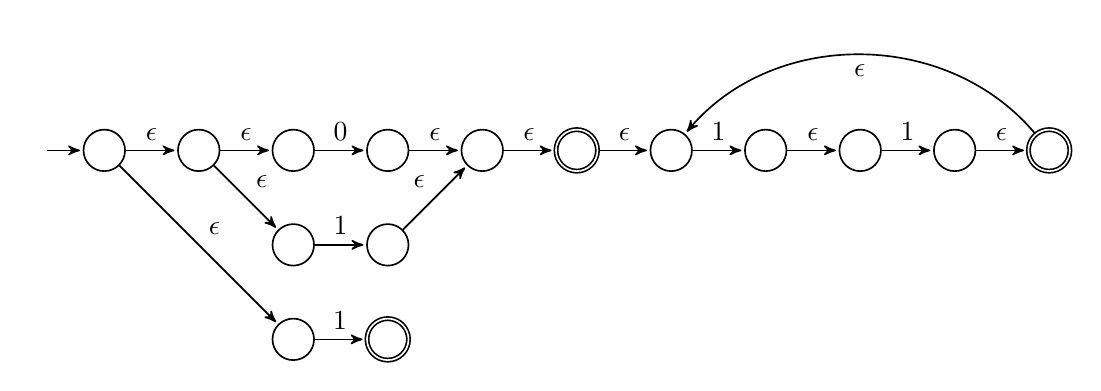
\begin{tikzpicture}[->,>=stealth',shorten >=1pt,auto,node distance=1.2cm, semithick, initial text={}]
  
        \tikzstyle{every state}=[fill=white,draw=black,text=black, minimum size=15pt]
        
        \node[initial, state]   (13)                 {};

        \node[state]            (6)  [right of = 13] {};
        \node[state]            (7)  [right of = 6]  {};
        \node[state]            (8)  [below of = 7]  {};
        \node[state]            (12) [right of = 8]  {};
        \node[state]            (9)  [right of = 7]  {};
        \node[state]            (10) [right of = 9]  {};
         
        \node[accepting, state] (4)  [right of = 10] {};
        \node[state]            (0)  [right of = 4]  {};
        \node[state]            (1)  [right of = 0]  {};
        \node[state]            (2)  [right of = 1]  {};
        \node[state]            (3)  [right of = 2]  {};
        \node[accepting, state] (5)  [right of = 3]  {};

        \node[state]            (14) [below of = 8]  {};
        \node[accepting, state]            (15) [right of = 14] {}; 
   
        \path
        (13) edge node {$\epsilon$} (6)
        (13) edge node {$\epsilon$} (14)
        (14) edge node {$1$}        (15)

        (6)  edge node {$\epsilon$} (7)
        (6)  edge node {$\epsilon$} (8)
        (7)  edge node {$0$}        (9)
        (9)  edge node {$\epsilon$} (10)
        (8)  edge node {$1$}        (12)
        (12) edge node {$\epsilon$} (10)
        
        (10) edge node {$\epsilon$} (4)

        (4) edge node {$\epsilon$} (0)
        (0) edge node {$1$} (1)
        (1) edge node {$\epsilon$} (2)
        (2) edge node {$1$} (3)
        (3) edge node {$\epsilon$} (5)
        (5) edge [bend right=50] node {$\epsilon$} (0)
        ;    
    \end{tikzpicture}           
    }

\end{itemize}


\part{b}
\begin{itemize}
    \item{$a:$

    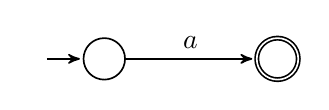
\begin{tikzpicture}[->,>=stealth',shorten >=1pt,auto,node distance=2.2cm, semithick, initial text={}]
  
    \tikzstyle{every state}=[fill=white,draw=black,text=black, minimum size=15pt]

    \node[initial,state]    (0)              {};
    \node[accepting, state] (1) [right of=0] {};
 
    \path (0) edge node {$a$} (1)
    ;                      
    \end{tikzpicture}    
    }
    \item{$b:$
        
    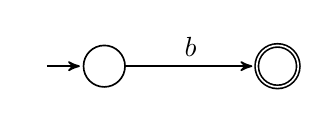
\begin{tikzpicture}[->,>=stealth',shorten >=1pt,auto,node distance=2.2cm, semithick, initial text={}]
  
    \tikzstyle{every state}=[fill=white,draw=black,text=black, minimum size=15pt]

    \node[initial,state]    (0)              {};
    \node[accepting, state] (1) [right of=0] {};
 
    \path (0) edge node {$b$} (1)
    ;                      
    \end{tikzpicture}                                          
    }
    \item{$c:$
        
    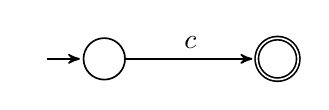
\begin{tikzpicture}[->,>=stealth',shorten >=1pt,auto,node distance=2.2cm, semithick, initial text={}]
  
    \tikzstyle{every state}=[fill=white,draw=black,text=black, minimum size=15pt]

    \node[initial,state]    (0)              {};
    \node[accepting, state] (1) [right of=0] {};
 
    \path (0) edge node {$c$} (1)
    ;                      
    \end{tikzpicture}        
    }
    \item{$d:$
        
    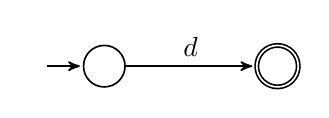
\begin{tikzpicture}[->,>=stealth',shorten >=1pt,auto,node distance=2.2cm, semithick, initial text={}]
  
    \tikzstyle{every state}=[fill=white,draw=black,text=black, minimum size=15pt]

    \node[initial,state]    (0)              {};
    \node[accepting, state] (1) [right of=0] {};
 
    \path (0) edge node {$d$} (1)
       
    ;                      
    \end{tikzpicture}    
    }
    \item{$c^*:$
        
    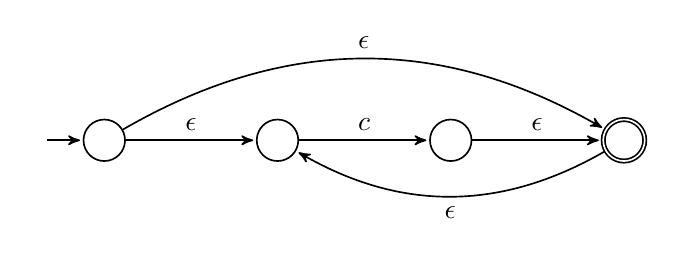
\begin{tikzpicture}[->,>=stealth',shorten >=1pt,auto,node distance=2.2cm, semithick, initial text={}]
  
    \tikzstyle{every state}=[fill=white,draw=black,text=black, minimum size=15pt]
    
    \node[initial, state]  (2)       {};
    \node[state]            (0) [right of = 2]  {};
    \node[state] (1) [right of = 0]  {};
    \node[accepting, state] (3) [right of = 1]  {};
    
    \path (2)  edge node {$\epsilon$} (0)
          (0)  edge node {$c$}        (1)
          (1)  edge node {$\epsilon$} (3)
          (3)  edge [bend left=30] node {$\epsilon$} (0)
          (2)  edge [bend left=30] node {$\epsilon$} (3)
    ;                      
    \end{tikzpicture}    
    }
    \item{$bc^*:$
         
    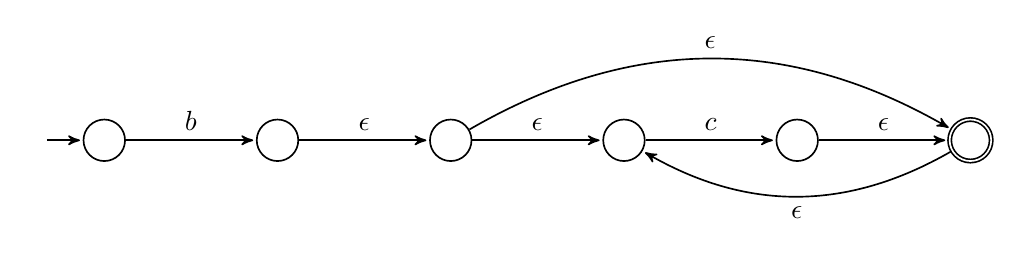
\begin{tikzpicture}[->,>=stealth',shorten >=1pt,auto,node distance=2.2cm, semithick, initial text={}]
  
    \tikzstyle{every state}=[fill=white,draw=black,text=black, minimum size=15pt]
    
    \node[initial, state]   (4)                 {};
    \node[state]            (5) [right of = 4]  {};
    \node[state]            (2) [right of = 5]  {};
    \node[state]            (0) [right of = 2]  {};
    \node[state]            (1) [right of = 0]  {};
    \node[accepting, state] (3) [right of = 1]  {};
    
    \path (2)  edge node {$\epsilon$} (0)
          (0)  edge node {$c$}        (1)
          (1)  edge node {$\epsilon$} (3)
          (3)  edge [bend left=30] node {$\epsilon$} (0)
          (2)  edge [bend left=30] node {$\epsilon$} (3)
          (4)  edge node {$b$} (5)
          (5)  edge node {$\epsilon$} (2)
    ;                      
    \end{tikzpicture}    

    }
    \item{$bc^*d:$
        
    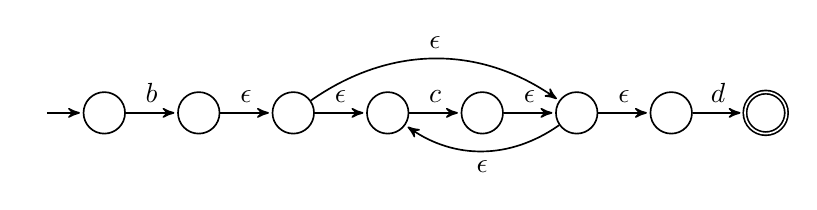
\begin{tikzpicture}[->,>=stealth',shorten >=1pt,auto,node distance=1.2cm, semithick, initial text={}]
  
    \tikzstyle{every state}=[fill=white,draw=black,text=black, minimum size=15pt]
    
    \node[initial, state]   (4)                 {};
    \node[state]            (5) [right of = 4]  {};
    \node[state]            (2) [right of = 5]  {};
    \node[state]            (0) [right of = 2]  {};
    \node[state]            (1) [right of = 0]  {};
    \node[state]            (3) [right of = 1]  {};
    \node[state]            (6) [right of = 3]  {};
    \node[accepting, state] (7) [right of = 6]  {};
    
    \path (2)  edge node {$\epsilon$} (0)
          (0)  edge node {$c$}        (1)
          (1)  edge node {$\epsilon$} (3)
          (3)  edge [bend left=35] node {$\epsilon$} (0)
          (2)  edge [bend left=35] node {$\epsilon$} (3)
          (4)  edge node {$b$} (5)
          (5)  edge node {$\epsilon$} (2)
          (3)  edge node {$\epsilon$} (6)
          (6)  edge node {$d$}        (7)
    ;
    \end{tikzpicture}    
    }
        
    \item{$a + bc^*d:$
        
    \begin{tikzpicture}[->,>=stealth',shorten >=1pt,auto,node distance=1.2cm, semithick, initial text={}]
  
    \tikzstyle{every state}=[fill=white,draw=black,text=black, minimum size=15pt]
    
    \node[initial, state]   (8)                 {};
    \node[state]            (9) [right of = 8]  {};
    \node[state]           (10) [right of = 9]  {};
    \node[accepting, state](11) [right of = 7]  {};
    \node[state]            (4) [above of = 8, right of = 8]  {};
    \node[state]            (5) [right of = 4]  {};
    \node[state]            (2) [right of = 5]  {};
    \node[state]            (0) [right of = 2]  {};
    \node[state]            (1) [right of = 0]  {};
    \node[state]            (3) [right of = 1]  {};
    \node[state]            (6) [right of = 3]  {};
    \node[state]            (7) [right of = 6]  {};
    
    \path (2)  edge node {$\epsilon$} (0)
          (0)  edge node {$c$}        (1)
          (1)  edge node {$\epsilon$} (3)
          (3)  edge [bend left=30] node {$\epsilon$} (0)
          (2)  edge [bend left=30] node {$\epsilon$} (3)
          (4)  edge node {$b$} (5)
          (5)  edge node {$\epsilon$} (2)
          (3)  edge node {$\epsilon$} (6)
          (6)  edge node {$d$}        (7)
          (8)  edge node {$\epsilon$} (4)
          (8)  edge node {$\epsilon$} (9)
          (9)  edge node {$a$}        (10)
          (10) edge node {$\epsilon$} (11)
          (7)  edge node {$\epsilon$} (11)
    ;
    \end{tikzpicture}    
    
    }

    \item{$(a + bc^*d)^*:$
         
    \begin{tikzpicture}[->,>=stealth',shorten >=1pt,auto,node distance=1.2cm, semithick, initial text={}]
  
    \tikzstyle{every state}=[fill=white,draw=black,text=black, minimum size=15pt]
    
    \node[initial, state]  (12)                 {};
    \node[accepting, state](13) [below of = 11] {};
    \node[state]            (8) [right of = 12] {};
    \node[state]            (9) [right of = 8]  {};
    \node[state]           (10) [right of = 9]  {};
    \node[state]           (11) [below of = 7, right of = 7]  {};
    \node[state]            (4) [above of = 8, right of = 8]  {};
    \node[state]            (5) [right of = 4]  {};
    \node[state]            (2) [right of = 5]  {};
    \node[state]            (0) [right of = 2]  {};
    \node[state]            (1) [right of = 0]  {};
    \node[state]            (3) [right of = 1]  {};
    \node[state]            (6) [right of = 3]  {};
    \node[state]            (7) [right of = 6]  {};
    
    \path (2)  edge node {$\epsilon$} (0)
          (0)  edge node {$c$}        (1)
          (1)  edge node {$\epsilon$} (3)
          (3)  edge [bend left=30] node {$\epsilon$} (0)
          (2)  edge [bend left=30] node {$\epsilon$} (3)
          (4)  edge node {$b$} (5)
          (5)  edge node {$\epsilon$} (2)
          (3)  edge node {$\epsilon$} (6)
          (6)  edge node {$d$}        (7)
          (8)  edge node {$\epsilon$} (4)
          (8)  edge node {$\epsilon$} (9)
          (9)  edge node {$a$}        (10)
          (10) edge node {$\epsilon$} (11)
          (7)  edge node {$\epsilon$} (11)
          (12) edge node {$\epsilon$} (8)
          (12) edge [bend right=30] node {$\epsilon$} (13)
          (13) edge [bend left=20] node {$\epsilon$} (8)
          (11) edge node {$\epsilon$} (13)
    ;
    \end{tikzpicture}    
    

    }
    \item{$(a + bc^*d)^*bc^*:$
         
    \begin{tikzpicture}[->,>=stealth',shorten >=1pt,auto,node distance=1.2cm, semithick, initial text={}]
  
    \tikzstyle{every state}=[fill=white,draw=black,text=black, minimum size=15pt]
   
    \node[state]           (14) [below of = 13] {};
    \node[state]           (15) [left of = 14]  {};
    \node[state]           (16) [left of = 15]  {};
    \node[state]           (17) [left of = 16]  {};
    \node[state]           (18) [left of = 17]  {};
    \node[accepting, state]           (19) [left of = 18]  {};

    \node[initial, state]  (12)                 {};
    \node[state]           (13) [below of = 11] {};
    \node[state]            (8) [right of = 12] {};
    \node[state]            (9) [right of = 8]  {};
    \node[state]           (10) [right of = 9]  {};
    \node[state]           (11) [below of = 7, right of = 7]  {};
    \node[state]            (4) [above of = 8, right of = 8]  {};
    \node[state]            (5) [right of = 4]  {};
    \node[state]            (2) [right of = 5]  {};
    \node[state]            (0) [right of = 2]  {};
    \node[state]            (1) [right of = 0]  {};
    \node[state]            (3) [right of = 1]  {};
    \node[state]            (6) [right of = 3]  {};
    \node[state]            (7) [right of = 6]  {};
    
    \path (2)  edge node {$\epsilon$} (0)
          (0)  edge node {$c$}        (1)
          (1)  edge node {$\epsilon$} (3)
          (3)  edge [bend left=30] node {$\epsilon$} (0)
          (2)  edge [bend left=30] node {$\epsilon$} (3)
          (4)  edge node {$b$} (5)
          (5)  edge node {$\epsilon$} (2)
          (3)  edge node {$\epsilon$} (6)
          (6)  edge node {$d$}        (7)
          (8)  edge node {$\epsilon$} (4)
          (8)  edge node {$\epsilon$} (9)
          (9)  edge node {$a$}        (10)
          (10) edge node {$\epsilon$} (11)
          (7)  edge node {$\epsilon$} (11)
          (12) edge node {$\epsilon$} (8)
          (12) edge [bend right=20] node {$\epsilon$} (13)
          (13) edge [bend left=10] node {$\epsilon$} (8)
          (11) edge node {$\epsilon$} (13)

          (13) edge [bend left=5] node {$\epsilon$} (14)
          (14) edge node {$b$} (15)
          (15) edge node {$\epsilon$} (16)
          (16) edge node {$\epsilon$} (17)
          (17) edge node {$c$} (18)
          (18) edge node {$\epsilon$} (19)
          (19) edge [bend right=50] node {$\epsilon$} (17)
          (16) edge [bend left=60]  node {$\epsilon$} (19)
    ;
    \end{tikzpicture}    
    


    }
\end{itemize}

\question{2}{}

\part{a} 

\par Describing each state with a regular expression with strings that take us to an acceptance state we can build the system:

\begin{center}
$
\begin{cases}
q_0 = \epsilon q_1 + bq_2 \\
q_1 = a q_1 + \epsilon q_2 + \epsilon \\
q_2 = \epsilon
\end{cases}
$
\end{center}

\begin{itemize}
    \item{Substitute $q_2$ into the second equation
    \begin{flalign*}
        q_1 &= a q_1 + \epsilon + \epsilon \\
            &= a^* \textup{ (by Arden's Lemma)}
    \end{flalign*}
    }

    \item{Substitute $q_1$ into the first equation
    \begin{flalign*}
       q_0 &= \epsilon a^* + b \epsilon \\
           &= a^* + b
    \end{flalign*}
    }
\end{itemize}

\par Since $q_0$ is the start state of the NFA, we have that the regular expression that describes this NFA is $a^* + b$.


\part{b}

\par Describing each state with a regular expression with strings that take us to an acceptance state we can build the system:

\begin{center}
$
\begin{cases}
q_0 = 0 q_1 + 1 q_2 + \epsilon \\
q_1 = 0 q_0 + 1 q_3 \\
q_2 = 0 q_3 + 1 q_0 \\
q_3 = 0 q_2 + 1 q_1
\end{cases}
$
\end{center}

\begin{itemize}
    \item{Substitute $q_1$ and $q_2$ into the last equation
    \begin{flalign*}
        q_3 &= 0 (0 q_3 + 1 q_0) + 1 (0 q_0 + 1 q_3) \\
            &= 00 q_3 + 01 q_0 + 10 q_0 + 11 q_3 \\
            &= (00 + 11) q_3 + (01 + 10) q_0 \\
            &= (00 + 11)^*(01 + 10) q_0 \textup{ (by Arden's Lemma)}
    \end{flalign*}
    }

    \item{Substitute $q_3$ into the second and third equation
    \begin{flalign*}
        q_1 &= 0 q_0 + 1 ((00 + 11)^* (01 + 10) q_0) \\
            &= 0 q_0 + 1 (00 + 11)^* (01 + 10) q_0   \\
            &= (1 (00 + 11)^* (01 + 10) + 0)q_0  \\
        \\
        q_2 &= 1 q_0 + 0 ((00 + 11)^* (01 + 10) q_0) \\
            &= 1 q_0 + 0 (00 + 11)^* (01 + 10) q_0   \\
            &= (0 (00 + 11)^* (01 + 10) + 1)q_0  
    \end{flalign*}
    }

    \item{Substitute $q_1$ and $q_2$ into the first equation
    \begin{flalign*}
        q_0 &= 0 ((1 (00 + 11)^* (01 + 10) + 0)q_0) + 1 ((0 (00 + 11)^* (01 + 10) + 1)q_0) \\
            &= (01 (00 + 11)^* (01 + 10) + 00)q_0 + (10 (00 + 11)^* (01 + 10) + 11)q_0 \\
            &= (01 (00 + 11)^* (01 + 10) + 00 + 10 (00 + 11)^* (01 + 10) + 11) q_0 \\
            &= ((01 + 10) (00 + 11)^* (01 + 10) + 00 + 11) q_0 \\
            &= ((01 + 10) (00 + 11)^* (01 + 10) + 00 + 11)^* \textup{ (by Arden's Lemma)} 
    \end{flalign*}
        
        }
\end{itemize}

\par Since $q_0$ is the start state of the NFA, we have that the regular expression that describes this NFA is $((01 + 10) (00 + 11)^* (01 + 10) + 00 + 11)^*$.





\question{3}{}

\part{a} $G = (V, \Sigma, R, S)$ where:
\begin{itemize}
    \item{$V = \{S\}$}
    \item{$\Sigma = \{a, b\}$}
\end{itemize}
    \par Note that $\epsilon \in L_1$, therefore our first rule is $S \rightarrow \epsilon$. To build other strings we have to add $1$'s into the end and twice this number of $0$'s at the beggining of the string, then the second rule is $S \rightarrow 00S1$.
\begin{itemize}
    \item {$R = \{S \rightarrow \epsilon$, $S \rightarrow 00S1\}$}
\end{itemize}


\part{b} $G = (V, \Sigma, R, S)$ where:

\begin{itemize}
    \item{$V = \{S\}$}
    \item{$\Sigma = \{a, b\}$}
\end{itemize}

\par Note that $\epsilon \in L_1$, therefore our first rule is $S \rightarrow \epsilon$. To build other strings of this language we have to guarantee that $m \geq n$ and keep $m$ and $n$ both odd or even. Which means that:

\par 1 $S \rightarrow aSb$; whenever adding an $a$ you have to add a new $b$ to keep $m \geq n$ and $m - n$ even.
\par 2 $S \rightarrow Sbb$; whenever adding a $b$ we need to add two of them to keep $m - n$ even.
\par Therefore the rules for this language are:

\begin{itemize}    
    \item{$R = \{S \rightarrow \epsilon$, $S \rightarrow Sbb$, $S \rightarrow aSb\}$}
\end{itemize}


\part{c} $G = (V, \Sigma, R, S)$ where:

\begin{itemize}
    \item{$V = \{S, S_1, R_1, T_1, S_2, R_2, T_2\}$}
    \item{$\Sigma = \{a, b, c, d\}$}
\end{itemize}
    
\par Note that the equation $m + n = p + q$ means that for every $a$ or $b$ added we need to add a new $c$ or $d$. To do that we are going to build the string from the outside to inside adding for every $a$ or $b$ a new $d$ or a new $c$. You should also note that it's hard have the pair of rules "for every $a$ add a new $c$" and "for every $b$ add a new $d$" because they intersect each other; to deal with this we are going to create rules for two different situations: $m \geq q$ and $m \leq q$.
\par In the case where $m \geq q$ we are looking for the language $L_1 = \{a^mb^nc^pd^q$ $|$ $m + n = p + q$, $m \geq q\} $ generate the strings with the following rules:
\par 1 $S_1 \rightarrow aS_1d | R_1$
\par 2 $R_1 \rightarrow aR_1c | T_1$
\par 3 $T_1 \rightarrow bT_1c | \epsilon$
\par We do not need a rule that adds a new $d$ when adding a $b$ because we assumed that $m \geq q$ therefore every $d$ of a string would already have been added by rule 1.
\par In the case where $m \leq q$ we are looking for the language $L_2 = \{a^mb^nc^pd^q$ $|$ $m + n = p + q$, $m \leq q\} $ generate the strings with the following rules:
\par 4 $S_2 \rightarrow aS_2d | R_2$
\par 5 $R_2 \rightarrow bR_2d | T_2$
\par 6 $T_2 \rightarrow bT_2c | \epsilon$
\par Simmilarly we do not need a rule that adds a new $c$ when adding a $a$ because we assumed that $m \leq q$ therefore every $a$ of a string would already have been added by rule 4.
    Now the last rule we need is the one that makes the union of $L_1$ and $L_2$: 
\par 7 $S \rightarrow S_1 | S_2$

\begin{itemize}    
    \item{$R = \{S \rightarrow S_1 | S_2$, 
        $S_1 \rightarrow aS_1d | R_1$,
        $R_1 \rightarrow aR_1c | T_1$,
        $T_1 \rightarrow bT_1c | \epsilon$,
        $S_2 \rightarrow aS_2d | R_2$,
        $R_2 \rightarrow bR_2d | T_2$,
        $T_2 \rightarrow bT_2c | \epsilon\}$
      }
\end{itemize}




\question{4}{}
$G = (V, \Sigma, R, S)$ where:
\begin{itemize}
    \item{$V = \{S, R\}$}
    \item{$\Sigma = \{a, b, *, (, ), +, \varepsilon \}$}; to avoid ambiguity we are going to use the symbol $\varepsilon$ to represent the empty string in the regular expressions we want to build.
\end{itemize}

\par To create all the regular expressions we are going to use two different variables: $R$ and $S$. The variable $S$ represents any non-empty regular expression while $R$ can be either $S$ or the empty string $\epsilon$.

\par 1 $S \rightarrow aR$
\par 2 $S \rightarrow bR$
\par 3 $S \rightarrow \varepsilon R$
\par 4 $S \rightarrow S^*R$
\par 5 $S \rightarrow (S)R$
\par 6 $S \rightarrow S + S$
\par 7 $R \rightarrow S$
\par 8 $R \rightarrow \epsilon$
\begin{itemize}    
    \item{$R = \{
        S \rightarrow aR, 
        S \rightarrow bR, 
        S \rightarrow \varepsilon R,
        S \rightarrow S^*R, 
        S \rightarrow (S)R,
        S \rightarrow S + S,
        R \rightarrow S,
        R \rightarrow \epsilon
    \}$
    }
\end{itemize}

\end{document}
